\documentclass[12pt,letterpaper]{exam}
%\usepackage{color}
\usepackage[usenames,dvipsnames,svgnames,table]{xcolor}
\usepackage[margin=0.9in]{geometry}
\renewcommand{\familydefault}{\sfdefault}
\usepackage{multicol}
\pagestyle{head}
\definecolor{c02}{HTML}{FFBBBB}
\definecolor{c03}{HTML}{FFDDDD}
\header{AM 108 Problem Set 04}{}{{\colorbox{c02}{\makebox[3.0cm][l]{Due Fri Feb 25}}}\\ at noon p.\thepage}
\runningheadrule
\headrule
\usepackage{diagbox}
\usepackage{graphicx} % more modern
%\usepackage{subfigure} 
\usepackage{amsmath} 
\usepackage{amssymb} 
%\usepackage{gensymb} 
%\usepackage{natbib}
\usepackage{hyperref}
%\usepackage{enumitem}
%\setlength{\parindent}{0pt}
%\usepackage{setspace}
%\pagestyle{empty}  
%\newcommand{\Sc}[0]{
%{\color{BlueViolet}\S}
%}
\usepackage{tcolorbox}
\usepackage[framed,numbered,autolinebreaks,useliterate]{mcode}

% \renewcommand{\labelenumii}{\theenumii}
% \renewcommand{\theenumii}{\theenumi-\arabic{enumii}.}

\newif\ifprintselans
\printselanstrue
%\printselansfalse
\newenvironment{selans}
{\ifprintselans
   \printanswers
   \renewcommand{\solutiontitle}{\noindent\textbf{Answer:}\par\noindent}
 \fi
}
{}

\newif\ifprintselsol
%\printselsoltrue
\printselsolfalse
\newenvironment{selsol}
{\ifprintselsol
   \printanswers
   \renewcommand{\solutiontitle}{\noindent\textbf{Solution:}\par\noindent}
 \fi
}
{}


\begin{document}
 \pdfpageheight 11in 
  \pdfpagewidth 8.5in

\noindent\textbf{Problem Set Instructions:}  
\begin{itemize}
\itemsep0pt
\item In your first attempt of the problem set problems, you are encouraged to treat the problem set as an open-notes quiz.  Work on it without consulting classmates, Ed, course staff, other people, other internet resources, or any solutions or answers.  Work on each problem, completing as much as you are able to, and making a note in your work whenever you become stuck or confused.
\item After your initial individual attempt, collaboration is encouraged (see guidelines below) as you continue to work on the problems.  You'll submit a pdf of this work as part of your problem set submission on Gradescope (and will also submit it on Canvas).
\item Submit the pdf of your problem set work with the problems written up in order (computational work should be included: it can be at the end of the pdf) on Canvas and access the solutions.
\item Complete the reflection questions below, and submit that reflection work, along with your problem set pdf, on Gradescope.
\end{itemize}
  
\noindent\textbf{Submission Instructions:}  
\begin{itemize}
\item Following the instructions above, upload a pdf of your work to Canvas.  Upload your reflection answers and the pdf to Gradescope.
\item If you would like to use mathematical software other than Mathematica, that's fine. 
\end{itemize}

\noindent\textbf{Late Work Policy:}
\begin{itemize}
\itemsep0pt
\item Problem sets are accepted up to eight hours late with no penalty (8pm Friday). 
\item Three 36 hour late days are available to every student (three extensions to 8pm on Saturday).  These late days are expected to be used for unexpected illness or other conflicts.
\item Additional late days are not typically 
available.
\item Problem sets are not accepted beyond the late deadline.
\end{itemize}

\noindent\textbf{Collaborating on Problem Sets:}  

\noindent Collaborating with classmates in planning and designing solutions to homework problems is encouraged.  Collaboration, cooperation, and consultation can all be productive.  Work with others to: 
\begin{multicols}{2}
\begin{itemize}
\itemsep-0.2em
    \item discuss the problem
    \item brainstorm
    \item walk through possible strategies
    \item outline solution methods
\end{itemize}   
\end{multicols}

\noindent For homework, you may consult or use:
\begin{multicols}{2}
\begin{itemize}
\itemsep-0.2em
    \item Course text (including answers in back)
    \item Your notes (taken during class)
    \item Class notes of other students
    \item Course handouts
    \item Canvas posts/Ed posts
    \item Computational tools such as Python, Mathematica, or Desmos
    \item Calculators
    \item Other books
    \item the Internet
\end{itemize}
\end{multicols}

\noindent You may:
\begin{itemize}
    \item Look at communal work while writing up your own solution
\end{itemize}

\noindent You may \textbf{not}:
\begin{itemize}
\itemsep-0.2em
    \item Look at the individual work of others while writing up your own solutions
    \item Post about problems online
\end{itemize}


\noindent Do \textbf{not} consult the following resources until after you think you have solved a problem, have fully written up your answer, and have submitted a pdf of your work to Canvas.
%\begin{multicols}{2}
\begin{itemize}
\itemsep-0.2em
    \item The text solution manual
    \item The posted solutions
    \item Other solutions (from previous years, from sites like Chegg or Math Stackexchange, etc)
\end{itemize}
%\end{multicols}


%\eject


% \begin{enumerate}
% \item Reflection questions

\section*{Reflection questions}
Submit these on Gradescope.
\begin{enumerate}
\item \begin{enumerate}
    \itemsep0pt
    \item When you worked on the problems individually, how did each problem go?
    \item Where did you get stuck or confused?  For any subpart where you were stuck or confused be specific.  \emph{For example 'I tried to use the hint for 3b, but I couldn't find a way to relate $r$ and $x$'.}
    \item What additional progress were you able to make when you consulted other people or additional resources?
    \item For each part of each problem, how did your work compare with the posted solution?  Identify similarities and differences.
\end{enumerate}  
\item For any problems you were not able to complete, what made them difficult to complete?  What did you learn from the posted solution?
\item What aspects of the course challenged you this week?  What did you do to address those challenges?  What topics/ideas/procedures do you not yet understand?
\item What did you understand the best this week?  What, if anything, do you understand better this week than you did in the past?
\item List the people that you worked with or consulted on the problem set problems.  This might include other students in the course, course instructors, or people who have previously taken the course.
\item Below, indicate how much of your time for this class has been doing the following activities:
	\begin{enumerate}
	\item Working on problem set problems or other practice problems alone
	\item Viewing preclass materials or reviewing course materials, including problem set solutions, alone
	\item Working on problem sets, reviewing notes, or discussing course topics with your classmates
	\item Working through supplementary materials
	\item Going to office hours
	\item Other (please specify)
	\end{enumerate}

\end{enumerate}


\section*{Problems}


\begin{questions}

\question (inspired by 6.1.4) Let $\dot{x} = y, \dot{y} = x(1+y)-1$.  
\begin{parts}
\item Find the fixed points of this system and classify them.  Sketch the nullclines (the $\dot{x} = 0$ curves, as well as the $\dot{y} = 0$ curves), the vector field, and a possible phase portrait.  Sketch phase portraits for $-3<x,y<3$.  Your hand-drawn phase portrait should show the linear behavior that you've found for any fixed points and then should link these linear pictures together so that no trajectories cross.

Tackle the phase portrait by hand, without using any numerical tools to draw it.

\begin{solution}
The nullclines are given by $y = 0$ for vertical motion and by $x(1+y) - 1 = 0$ for horizontal motion, so $y = -1 + 1/x$.  There is neither horizontal nor vertical motion when $y = 0$, $x = 1$, so that's the fixed point (there is only one).

The Jacobian is $\left(\begin{array}{c c} 0 & 1 \\ (1+y) & x \end{array}\right)$ so at the fixed point it is $\left(\begin{array}{c c} 0 & 1 \\ 1 & 1 \end{array}\right)$.  The trace is $1$ and the determinant is $-1$ so this is a saddle point.

The eigenvalues are given by $\tau/2 \pm \frac{1}{2}\sqrt{\tau^2 - 4\Delta} = \frac{1}{2}(1 \pm \sqrt{5})$.

The eigenvectors are given by $\left(\begin{array}{c c} 0 & 1 \\ 1 & 1 \end{array}\right)\left(\begin{array}{c} a \\ b\end{array}\right) = \lambda_{\pm}\left(\begin{array}{c} a \\ b\end{array}\right)$.  So $b = \lambda_{\pm} a$ and the eigenvectors are $\left(\begin{array}{c} 1 \\ \lambda_{\pm} \end{array}\right)$.  The stable one is $\left(\begin{array}{c} 1 \\ (1-\sqrt{5})/2 \end{array}\right) \approx \left(\begin{array}{c} 1 \\ -0.1 \end{array}\right)$ and the unstable one is $\left(\begin{array}{c} 1 \\ (1+\sqrt{5})/2 \end{array}\right) \approx \left(\begin{array}{c} 1 \\ 2.1 \end{array}\right)$.

Once I draw this information in, I put a representative vector in each sector (where I think of the nullclines as splitting the region into sectors).

%\includegraphics[width=0.5\linewidth]{AM108F19pset04p1.png}
%\includegraphics[width=0.5\linewidth]{AM108F19pset04p2.png}

To draw the phase portrait, I extend each of the stable / unstable manifolds of the fixed point.  I also draw a trajectory that crosses each nullcline and think about how it would bend next.  That's enough to get an idea of things!

%\includegraphics[width=0.7\linewidth]{AM108F19pset04p3.png}

\end{solution}


\item Make two phase portraits using computational tools, one for $-3<x,y<3$ and one for $-30<x,y<30$.  

\emph{Using Python's or Mathematica's \texttt{StreamPlot}, or another tool is just fine, but cite it here and explain your setup.}

\begin{solution}
I'll make my phase portraits in Mathematica, by putting the vector field $y\vec i + (x(1+y)-1)\vec j$ into the streamplot command.

\begin{verbatim}
smallphaseportrait = 
 StreamPlot[{y, x (1 + y) - 1}, {x, -3, 3}, {y, -3, 3}, 
  PerformanceGoal -> "Quality", FrameLabel -> {x, y}, 
  LabelStyle -> Medium]
nullclines = 
  Plot[{0, -1 + 1/x}, {x, -3, 3}, PlotRange -> {{-3, 3}, {-3, 3}}];
Show[smallphaseportrait, nullclines, Graphics[Circle[{1, 0}, 0.13]]]
\end{verbatim}

Here's the small one, with the nullclines and the little circle to indicate the unstable fixed point (plot on left):

%\includegraphics[width=3in]{AM108F19pset04p4} 
%\includegraphics[width=3in]{AM108F19pset04p5}

I added the stable and unstable manifolds to the plot on the right (see my Mathematica code: to do this I integrated forward in time to find trajectories paralleling the unstable ones.  I integrated backward in time to find trajectories close to the stable ones).



\eject

\begin{verbatim}
f[x_, y_] = {y, x (1 + y) - 1};
largephaseportrait = 
  StreamPlot[f[x, y], {x, -30, 30}, {y, -30, 30}, 
   PerformanceGoal -> "Quality", FrameLabel -> {x, y}];
nullclines = 
  Plot[{0, -1 + 1/x}, {x, -30, 30}, 
   PlotRange -> {{-30, 30}, {-30, 30}}];
Show[largephaseportrait, nullclines, Graphics[Circle[{1, 0}, 0.5]]]
\end{verbatim}

I just change the domain (and the circle size) to make the large phase portrait.  I am still including the nullclines for reference.

%\includegraphics[width=3in]{AM108F19pset04p6} 

I add the stable and unstable manifolds to this one, too.



\end{solution}


\item On the $-30<x,y<30$ phase portrait, there are a few features of the flow that become visible.  
\begin{itemize}
    \item Find a way to approximate the quadratic curves formed by trajectories that pass through $x=0$ (and that are present whenever $\vert y\vert$ is sufficiently large).
    
    \emph{To think about these curves, recall that trajectories are tangent to the vectors of the vector field.  The slope of the vectors and the slope of the trajectories is locally the same. Approximate $\displaystyle\frac{dy/dt}{dx/dt}$.  This gives you an expression for $\displaystyle\frac{dy}{dx}$. Go from there - it should integrate nicely.}
    
    \item Explain the existence of the somewhat vertical trajectories.
    
    \item Identify the curve that many trajectories approach in forwards time (for $x\ll -1$) or in backwards time (for $x\gg 1$). 
\end{itemize}

\begin{solution}

\textbf{Parabolas}

The slope of a trajectory is given by $\frac{dy}{dx} = \frac{\dot{y}}{\dot{x}}  = (x(1+y) - 1)/y$, so $\frac{dy}{dx} = x + \frac{x-1}{y}$.  For large enough $y$ and small enough $x$ this can be approximated as $\frac{dy}{dx}\approx x$, so $y \approx \frac{1}{2} x^2 + c$ where $c$ is an arbitrary constant.  This yields parabolas that open upwards.


I will plot the parabolas on the phase portrait (for a number of different initial conditions / values of the constant $c$):
\begin{verbatim}
parabolas = {};
For[constant = 30, constant >= -30, constant = constant - 10,
 p2 = Plot[x^2/2 + constant, {x, -30, 30}, PlotStyle -> Green];
 AppendTo[parabolas, p2];
 ]
For[constant = -80, constant > -1000, constant = constant - 80,
 p2 = Plot[x^2/2 + constant, {x, -30, 30}, PlotStyle -> Blue];
 AppendTo[parabolas, p2];
 ]
Show[largephaseportrait, parabolas]
\end{verbatim}
%\includegraphics[width=3in]{AM108F19pset04p7} 


These parabolas do an absurdly good job of capturing the shape of the trajectories, so long as we're not too close to $y = 0$.  Notice that the shapes are completely unrelated to the direction of time: in some places we travel upward on the parabola and in other places downward.  So approximating $\frac{dy}{dx}$ was able to capture the shapes, but not the actual dynamics.


\textbf{Vertical trajectories}

$\frac{dy}{dx} = x + \frac{x-1}{y}$.  For large $x$ this number is large (either large and negative or large and positive), so the slope of the trajectories will be large meaning the trajectories are somewhat vertical.

\textbf{Curve that is approached}

It looks like we approximately approach the curve $y=0$ both in forwards and in backwards time (just based on looking at the plot).  The curve appears to correspond to horizontal motion.  The motion will be purely horizontal along the $\dot{y} = 0$ nullcline, so when $y = -1 + \frac{1}{x}$.  For $x$ away from $0$, this is approximately the curve $y = -1$.

Looking in forwards time, on the left half of the phase portrait where $ x < 0$, trajectories are pushed downward if they are above this nullcline and upward if they are below it, so they are pushed close to the nullcline.  

In backwards time, something similar happens on the right half of the phase portrait.


%\includegraphics[width=3in]{AM108F19pset04p10} 
\end{solution}
\end{parts}

\question (inspired by 6.1.14 and 6.4.6) Consider the two species model \begin{align*}\dot{N_1} = & r_1 N_1 (s_{11}-N_1) - s_{21} N_1 N_2 \\ \dot{N_2} = & r_2 N_2(s_{22}-N_2) - s_{12} N_1N_2.\end{align*}

\begin{parts}
\item Show the steps needed to nondimensionalize this to 
\begin{align*}\dot{x} = &  x (1-x) - \beta_{1} x y \\ \dot{y} = & \rho y(1-y) - \beta_2 x y.\end{align*}

Provide formulas for $A_1, \ A_2,$ $T$, $\rho,\beta_1,\beta_2$ where $N_1 = xA_1$ and $N_2 = yA_2$.

\emph{Depending on the two species that are interacting, it may be appropriate to use the same constant $A_1$ for nondimensionalization of both species, or to use different constants for each.  For this problem, use different constants for each.}

\begin{solution}
To nondimensionalize, create new nondimensional variables: $x = N_1/A_1$, $y = N_2/A_2$, $\tau = t / T_0$.

Then substitute into the system: 

$\displaystyle\left\{\begin{array}{l} \frac{dxA_1}{d\tau T_0} =  r_1 A_1 x (1-x A_1/K_1) - \alpha_1 A_1 A_2 x y \\  \frac{dy A_2}{d\tau T_0} =  r_2 A_2 y(1-yA_2/K_2) - \alpha_2A_1 A_2 xy\end{array}\right.$

Multiply through by the dimensional constants so that the left hand side is nondimensional:

$\left\{\begin{array}{l} \frac{dx}{d\tau} =  r_1T_0 x (1-x A_1/K_1) - \alpha_1 T_0 A_2 x y \\  \frac{dy}{d\tau} =  r_2 T_0 y(1-yA_2/K_2) - \alpha_2A_1 T_0 xy\end{array}\right.$

I can now identify the six nondimensional groups: 

$r_1 T_0$, $A_1/K_1$, $\alpha_1 T_0 A_2$, $r_2 T_0$, $A_2/K_2$, $\alpha_2A_1T_0$.

I will eliminate three of them by selecting $A_1, A_2, T_0$ and the other three will become parameters.

I'll choose to eliminate both carrying capacities, and one of the growth rate terms.  Let $A_2 = K_2$, $A_1 = K_1,  T_0 = 1/r_1$.  Substituting these into the nondimensional groups, let $\beta_1 = \alpha_1 K_2 / r_1$, $\rho = r_2/r_1$, $\beta_2 = \alpha_2 K_1/r_1$.


The system becomes

$\left\{\begin{array}{l} \frac{dx}{d\tau} =   x (1-x ) - \beta_1 x y \\  \frac{dy}{d\tau} =  \rho y(1-y) - \beta_2 xy\end{array}\right.$

\end{solution}

\item Analyze the system, showing your analysis.  Show that there are four qualitatively different phase portraits in terms of the long term behavior of the system and identify the long term behavior in each case.

\emph{To help guide your work, nullclines for the four qualitatively different cases are shown below.}

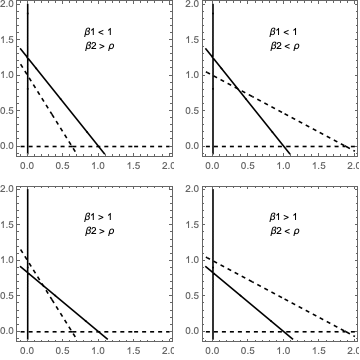
\includegraphics{img/PS04competition.png}

\begin{itemize}
    \item For more insight into this model, watch the following video about this model by Professor Kate Meyer: \url{https://www.youtube.com/embed/cH52VRuVKkw}
    \item Three of the fixed points have straightforward expressions.  For the fourth, I found it helpful to name it $(x^*,y^*)$, rather than always expressing it in terms of parameters of the system.
    \item If you choose to use the trace and determinant for your classification, the Mathematica/Python  \texttt{simplify} command can help simplify the output.
    \item Notice that in two of the cases the $(x^*,y^*)$ fixed point is not in the 1st quadrant (so does not need to be classified).
    \item If you have inequalities $a<b$ and $c<d$ (for $a,b,c,d>0$), then $ac<bd$.  This can be a helpful fact to use to classify the $(x^*,y^*)$ fixed point algebraically.
    \item If you are stuck in any  manipulations post to Ed.
\end{itemize}

\begin{solution}

To analyze the system, I'll start by factoring the right hand side of each equation.

$\left\{\begin{array}{l} \frac{dx}{d\tau} =   x\left( (1-x ) - \beta_1  y\right) \\  \frac{dy}{d\tau} =  y\left(\rho (1-y) - \beta_2 x\right)\end{array}\right.$

Fixed points occur when $x = 0$ or $1-x - \beta_1 y = 0$ and when $y = 0$ or $\rho(1-y) - \beta_2 x = 0$.

There are four possible combinations:
\begin{enumerate}
\item $x = 0, y = 0$ so the fixed point is $(0,0)$.
\item  $1 - x - \beta_1 y = 0, y = 0$, so the fixed point is $(1,0)$
\item   $x = 0$, $\rho(1-y)-\beta_2 x = 0$, so the fixed point is $(0,1)$
\item  $1-x-\beta_1 y = 0, \rho(1-y) - \beta_2 x = 0$.  Call the location of this fixed point $(x^*, y^*)$.  We have $\displaystyle x^* = \frac{\rho(\beta_1 - 1)}{\rho - \beta_1 \beta_2}$.  $\displaystyle y^* = \frac{\beta_2 - \rho}{\rho - \beta_1 \beta_2}$.  We only care about nonnegative $x^*$ and $y^*$, so this fixed point is only of interest when $\beta_2 - \rho, \rho - \beta_1\beta_2, \beta_1 - 1$ all have the same sign.
\end{enumerate}

Next I'll look at their stability, since that is likely to vary across the qualitative cases.  First I'll find the Jacobian.  When I do this, I'll use the product rule and preserve the factored expressions.  That will make subbing in the different fixed point conditions a bit easier:

\[\left(\begin{array}{c c} f_x & f_y \\ g_x  & g_y \end{array}\right) = \left(\begin{array}{c c} (1-x-\beta_1 y) - x & -\beta_1 x \\ -\beta_2 y & (\rho(1-y) - \beta_2 x) - \rho y  \end{array}\right) \]

For the four fixed points:
\begin{enumerate}
\item $x = 0, y = 0$ so the fixed point is $(0,0)$ and the Jacobian is $\left(\begin{array}{c c} 1 & 0 \\ 0 & \rho  \end{array}\right) $
\item  $1 - x - \beta_1 y = 0, y = 0$, so the fixed point is $(1,0)$.  Substituting these conditions into the Jacobian, it reduces to $\left(\begin{array}{c c}  - x & -\beta_1 x \\ -\beta_2 y & (\rho(1-y) - \beta_2 x)  \end{array}\right)$.  Letting $x = 1$ and $y = 0$, this becomes $\left(\begin{array}{c c}  -1 & -\beta_1 \\ 0 & \rho - \beta_2  \end{array}\right)$
\item   $x = 0$, $\rho(1-y)-\beta_2 x = 0$, so the fixed point is $(0,1)$. Substituting these conditions into the Jacobian, it reduces to $\left(\begin{array}{c c} (1-x-\beta_1 y) & -\beta_1 x \\ -\beta_2 y & - \rho y  \end{array}\right) $.  Letting $x =0$ and $y=1$, this becomes $\left(\begin{array}{c c} 1-\beta_1 & 0 \\ -\beta_2 & - \rho   \end{array}\right).$  There is a symmetry between this fixed point and the $(1,0)$ fixed point.  $1$ and $\rho$ have analogous roles and $\beta_1$ and $\beta_2$ have analogous roles.

\item  $1-x-\beta_1 y = 0, \rho(1-y) - \beta_2 x = 0$.  The fixed point is $(x^*, y^*)$.  Substituting these conditions into the Jacobian, it reduces to $\left(\begin{array}{c c}  - x & -\beta_1 x \\ -\beta_2 y & - \rho y  \end{array}\right) $.  Letting $x=x^*$, $y=y^*$, this becomes $\left(\begin{array}{c c}  - x^* & -\beta_1 x^* \\ -\beta_2 y^* & - \rho y^*  \end{array}\right) $
\end{enumerate}

%\vfill

Now I'm ready to find the trace and determinant and to start classifying the fixed points.

\begin{tabular}{c | c| c| c| c}
f.p. & Jacobian & trace & determinant & trace \\
\hline
$(0,0)$ & $\left(\begin{array}{c c} 1 & 0 \\ 0 & \rho  \end{array}\right) $ & $\tau = 1+\rho$ & $\Delta = \rho$ & $\tau = 1 + \Delta$ \\
\hline
 $(1,0)$ & $\left(\begin{array}{c c}  -1 & -\beta_1 \\ 0 & \rho - \beta_2  \end{array}\right)$ & $\tau = -1 + \rho - \beta_2$ & $\Delta = -(\rho - \beta_2)$ & $\tau = -1 -\Delta$ \\
 \hline
 $(0,1)$ & $\left(\begin{array}{c c} 1-\beta_1 & 0 \\ -\beta_2 & - \rho   \end{array}\right).$ & $\tau = 1-\beta_1 - \rho$ & $\Delta = -\rho(1-\beta_1)$ & $\tau = -\frac{\Delta}{\rho} - \rho$ \\
\hline
 $(x^*,y^*)$ & $\left(\begin{array}{c c}  - x^* & -\beta_1 x^* \\ -\beta_2 y^* & - \rho y^*  \end{array}\right) $ & $\tau = -x^* - \rho y^*$ & $\Delta = (\rho -\beta_1\beta_2) x^*y^*$
\end{tabular}
\vfill

%\eject 

I'll look at the determinant to distinguish between saddle points and repellers/attractors.  When the determinant is negative I'll ignore the trace.  When it is positive I will classify repeller vs attractor based on the sign of the trace.  Recall that all constants are nonnegative, as are $x$ and $y$.  I've written the trace in terms of the determinant, when I can, to make classifying easier.

\begin{tabular}{c | c| c| c}
f.p. &  determinant & trace & type\\
\hline
$(0,0)$ &   $\Delta = \rho$ & $\tau = 1 + \Delta$  & $\rho > 0$ so repeller\\
\hline
 $(1,0)$ & $\Delta = -(\rho - \beta_2)$ & $\tau = -1 -\Delta$ & $\left\{\begin{array}{c} \rho > \beta_2: \text{ saddle pt} \\ \rho < \beta_2: \text{ attractor}\end{array}\right.$ \\
 \hline
 $(0,1)$ & $\Delta = -\rho(1-\beta_1)$ & $\tau = -\frac{\Delta}{\rho} - \rho$ & $\left\{\begin{array}{c} 1 > \beta_1: \text{ saddle pt} \\ 1 < \beta_1: \text{ attractor}\end{array}\right.$ \\
\hline
 $(x^*,y^*)$ &  $\Delta = (\rho -\beta_1\beta_2) x^*y^*$&  $\tau = -x^* - \rho y^*$ & $\left\{\begin{array}{c} \rho < \beta_1\beta_2: \text{ saddle pt} \\ \rho > \beta_1\beta_2: \text{ attractor}\end{array}\right.$
\end{tabular}

Four clear cases have arisen based on $1$ vs $\beta_1$ and $\rho$ vs $\beta_2$.

\begin{enumerate}
\item $1<\beta_1$, $\rho < \beta_2$, so $\rho < \beta_1\beta_2$.  $(0,0)$ is a repeller.  $(1,0)$ is an \textbf{attractor}.  $(0,1)$ is an \textbf{attractor}.  $(x^*,y^*)$ is a saddle point.
\item $1<\beta_1$, $\rho > \beta_2$, so $\rho\text{ ? }\beta_1\beta_2$.  $(0,0)$ is a repeller.  $(1,0)$ is an \textbf{attractor}.  $(0,1)$ is a saddle point.  $\beta_1 -1$ and $\beta_2 - \rho$ have different signs so the $(x^*,y^*)$ fixed point is out of range.
\item $1>\beta_1$, $\rho < \beta_2$, so $\rho\text{ ? }\beta_1\beta_2$.  $(0,0)$ is a repeller.  $(1,0)$ is a saddle point.  $(0,1)$ is an \textbf{attractor}.  $\beta_1 -1$ and $\beta_2 - \rho$ have different signs so the $(x^*,y^*)$ fixed point is out of range.
\item $1>\beta_1$, $\rho > \beta_2$, so $\rho > \beta_1\beta_2$.  $(0,0)$ is a repeller.  $(1,0)$ is a saddle point.  $(0,1)$ is a saddle point.  $(x^*,y^*)$ is an \textbf{attractor}.
\end{enumerate}

These are four scenarios!

We can go to 
\begin{enumerate}
\item a long term state of a single species where which species depends on initial conditions,
\item all one species for all initial conditions, 
\item all the other species for all initial conditions,  
\item or a long term state of coexistence.
\end{enumerate}



\end{solution}

\item Provide conditions under which the two species stably coexist.  Explain the biological meaning of these conditions.  

\begin{itemize}
    \item To explain the biological meaning, it can be helpful to think of carrying capacity as reflecting competition within a species, and the interaction terms as reflecting competition between species.  Watching the video link in the previous part may also be helpful here.
\end{itemize}

\begin{solution}

Coexistence is happening when $1 > \beta_1$ and $\rho > \beta_2$, so when the nondimensional growth rates are stronger than the nondimensional losses due to competition.  

In dimensional terms, $\beta_1 = \alpha_1 K_2/r_1$, so $r_1$, the nondimensional growth rate, is greater than $\alpha_1K_2$, the loss coefficient from competition ($\alpha_1$) weighted by some measure of how many of the competitors there are ($K_2$).

Similarly, we also need $r_2/r_1 > \alpha_2K_1/r_1$ so $r_2 > \alpha_2 K_1$, the growth rate of the second species needs to be larger than the loss coefficient from competition weighted by the amount of the competitor.

We are getting coexistence when competition has a sufficiently weak impact on both populations.  That makes sense: if the species weren't interacting at all, each one would have a population set by its carrying capacity, so there would be coexistence at $(K_1, K_2)$.

\end{solution}

\part (Optional: time permitting) $(1,0)$ is a saddle when $\rho>\beta_2$. Its stable manifold is the x-axis.  Its unstable manifold is a curve that is harder to find. The goal of this exercise is to approximate this unknown curve.
\begin{itemize}
\item Let $( x, y )$ be a point on the unstable manifold, and assume that $( x, y )$ is close to (1,0). Introduce a new variable $u=x-1$, so that the fixed point is at $(0,0)$ in $uy$-space.

Curves given by $\frac{dy}{du} = \frac{\dot y}{\dot u}$ lie along trajectories of the system.  When such curves pass through a saddle point in 2D, they must align with the stable or unstable manifold of the saddle.  See \href{https://math.libretexts.org/Bookshelves/Differential_Equations/Book%3A_Ordinary_Differential_Equations_(Wiggins)/06%3A_Stable_and_Unstable_Manifolds_of_Equilibria}{Wiggins example 6.13 for further explanation}

The stable manifold is given by $y = 0$, and we have $\dot y = 0$ so $\frac{dy}{du} = 0 = \frac{\dot y}{\dot u}$.

The unstable manifold is not trivial.  Write the unstable manifold as an unknown curve $y=a_1u+a_2u^2+O( u^3 )$.

To determine the coefficients $a_1$ and $a_2$, use $\frac{dy}{du} = \dot y/\dot u$ and also $\frac{dy}{du} = a_1 + 2a_2 u$.  Equate these.

\item Find $a_1$ by solving the $O(u)$ equation and $a_2$ by solving the $O(u^2)$ equation.  \emph{$a_1$ will be along the unstable eigenspace.}
\item Choose a parameter set and check that your analytical result produces a curve with the same shape as the unstable manifold close to the point $(1,0)$.

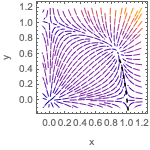
\includegraphics{img/PS04manifold.png}
\end{itemize}
\begin{solution}
See uploaded, handwritten notes.
\end{solution}
\end{parts}

\question (6.4.11) Vasquez and Redner (2004, p. 8489) mention a highly simplified model of political opinion dynamics consisting of a population of leftists, rightists, and centrists.  The leftists and rightists never talk to each other; they are too far apart politically to even begin a dialogue.  But they do talk to the centrists.  This is how opinion change occurs in the model.  Whenever an extremist of either type talks with a centrist, one of them convinces the other to change his or her mind, with the winner depending on the sign of the parameter $r$.  If $r>0$ the extremist always wins and persuades the centrist to move to that end of the spectrum.  If $r<0$ the centrists always wins and pulls the extremist to the middle.  The model's governing equations are
\begin{align*}
\dot{x}&= r x z \\
\dot{y}&=r y z\\
\dot{z}&=-rxz-ryz
\end{align*}
where $x$, $y$, and $z$ are the relative fractions of rightists, leftists, and centrists, respectively, in the population.
\begin{parts}
\item Show that the set $x+y+z = 1$ is invariant (i.e. $\frac{d}{dt}(x + y + z - 1) = 0$).  What does this invariant represent in the context of the model?
\begin{solution}
To show it is invariant I will take the time derivative: $\dot{x} + \dot{y} + \dot{z} = r x z + r y z - r x z - r y z = 0$.  $\frac{d}{dt}(x+y+z) = 0$ so $x+y+z$ is constant in time.  That means it is invariant (unchanging) under the action of the dynamical system.
\end{solution}
\item Use the invariant to reduce this to a two variable system from the three variable system. 
\begin{solution}
Eliminate $z$ from the system. $z = 1- x- y$, so $\dot{x} = rx (1-x-y)$ and $\dot{y} = r y (1-x-y)$.  Now we have a two-variable system.
\end{solution}
\item Analyze the long term behavior predicted by the model for both positive and negative values of $r$.
\begin{solution}
I will start by looking for fixed points:
$\dot{x} = 0$ when $x=0$ or $1-x-y = 0$.  $\dot{y} = 0$ when $ y = 0$ or $1 -x - y = 0$.  Fixed points are given by combinations of these:
\begin{itemize}
\item $x = 0$, $y = 0$ so $(0,0)$
\item $x = 0$, $1-x-y = 0$ so $(0,1)$
\item $1-x-y = 0$, $y = 0$ so $(1,0)$
\item $1 -x -y = 0$, $1-x-y = 0$. so the line $(x, 1-x)$ is a line of fixed points.  The $(0,1)$ and $(1,0)$ fixed points sit on this line.
\end{itemize}

Next I'll find the Jacobian to look at the stability: 

$\left(\begin{array}{c c }r(1-x-y) - rx & -rx \\ -ry & r(1-x-y) - ry \end{array}\right)$.

Substituting the fixed point cases:
\begin{itemize}
\item $x = 0$, $y = 0$ so $(0,0)$.  Jacobian is $\left(\begin{array}{c c }r & 0 \\ 0 & r \end{array}\right) = r I_2$ (where $I_2$ is the 2x2 identify matrix), so the eigenvalues are $\lambda = r, r$ and every vector is an eigenvector.
\item $1 -x -y = 0$, $1-x-y = 0$. so the line $(x^*, 1-x^*)$.  Jacobian is $\left(\begin{array}{c c }- rx^* & -rx^* \\ -ry^* & - ry^* \end{array}\right)$.  The trace is $-r (x^*+y^*)$ and the determinant is $0$.  There is a zero eigenvalue (which makes sense: it is a line of fixed points) and an eigenvalue with sign given by $-r$. To find the eigenvector, $\left(\begin{array}{c c }- rx^* & -rx^* \\ -ry^* & - ry^* \end{array}\right)\left(\begin{array}{c} a \\ b\end{array}\right) = -r(x^*+y^*)\left(\begin{array}{c} a \\ b\end{array}\right)$, so $-rx^*(a+b) = -r(x^*+y^*) a \Rightarrow ax^* + bx^* = ax^* + ay^* \Rightarrow b = ay^*/x^*$ and the eigenvector is $\left(\begin{array}{c} x^* \\ y^*\end{array}\right)$  

It looks like the lines $y = mx$ might be invariants under the action of the dynamical system.  Consider the line $y - m x = 0$.  On this line, $\dot{y} - m\dot{x} = r y(1-x-y) - m r x(1-x-y) = r(1-x-y)(y-mx) = 0$ (because $y-mx = 0$), so these lines through the origin are actually invariant.

%\includegraphics[width=.5\linewidth]{AM108F19pset04p9}
%\includegraphics[width=.5\linewidth]{AM108F19pset04p8}

For $r<0$, $x\rightarrow 0, y\rightarrow 0, z\rightarrow 1$ while for $r> 0$, given initial conditions $(x_0, y_0, 1-x_0-y_0)$, the flow will be along the line $y = \frac{y_0}{x_0} x$ until we hit $y = 1- x$, and $z \rightarrow 0$.

\end{itemize}

\end{solution}
\item Interpret the results in political terms.
\begin{solution}
When the centrist always wins ($r < 0 $) the rightists and leftists disappear from the system and centrists remain.

When the extremist always wins ($r>0$) the initial proportion of rightists and leftists sets the final proportion (the proportion stays the same at all times) while the centrists disappear.
\end{solution}

\end{parts}


 \end{questions}




\end{document}